\documentclass[border=6pt]{standalone}
\usepackage{tikz}
\usetikzlibrary{arrows.meta,positioning,calc,shapes.geometric,fit,backgrounds,patterns,matrix,decorations.pathreplacing}
\begin{document}
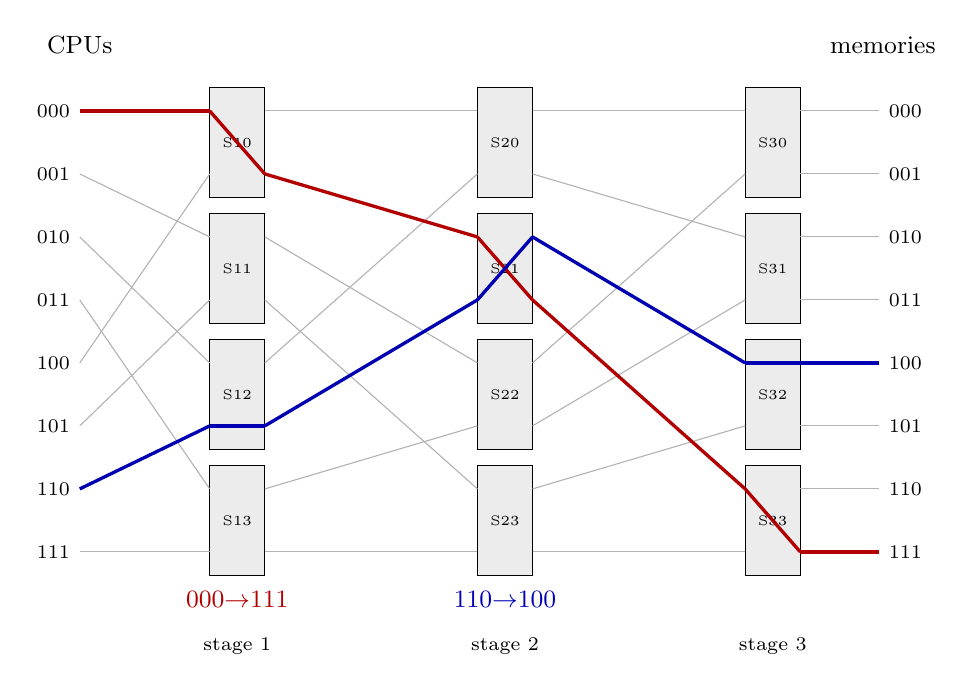
\begin{tikzpicture}[>=Stealth,font=\small]
%% route 0 7 [0, 1, 3, 7]
%% route 6 4 [6, 5, 2, 4]
\draw[fill=gray!15] (2.25,0.3) rectangle (2.95,-1.1);
\node[font=\tiny] at (2.6,-0.4) {S10};
\draw[fill=gray!15] (2.25,-1.3) rectangle (2.95,-2.7);
\node[font=\tiny] at (2.6,-2.0) {S11};
\draw[fill=gray!15] (2.25,-2.9000000000000004) rectangle (2.95,-4.3);
\node[font=\tiny] at (2.6,-3.6) {S12};
\draw[fill=gray!15] (2.25,-4.500000000000001) rectangle (2.95,-5.9);
\node[font=\tiny] at (2.6,-5.200000000000001) {S13};
\draw[fill=gray!15] (5.65,0.3) rectangle (6.35,-1.1);
\node[font=\tiny] at (6.0,-0.4) {S20};
\draw[fill=gray!15] (5.65,-1.3) rectangle (6.35,-2.7);
\node[font=\tiny] at (6.0,-2.0) {S21};
\draw[fill=gray!15] (5.65,-2.9000000000000004) rectangle (6.35,-4.3);
\node[font=\tiny] at (6.0,-3.6) {S22};
\draw[fill=gray!15] (5.65,-4.500000000000001) rectangle (6.35,-5.9);
\node[font=\tiny] at (6.0,-5.200000000000001) {S23};
\draw[fill=gray!15] (9.05,0.3) rectangle (9.75,-1.1);
\node[font=\tiny] at (9.4,-0.4) {S30};
\draw[fill=gray!15] (9.05,-1.3) rectangle (9.75,-2.7);
\node[font=\tiny] at (9.4,-2.0) {S31};
\draw[fill=gray!15] (9.05,-2.9000000000000004) rectangle (9.75,-4.3);
\node[font=\tiny] at (9.4,-3.6) {S32};
\draw[fill=gray!15] (9.05,-4.500000000000001) rectangle (9.75,-5.9);
\node[font=\tiny] at (9.4,-5.200000000000001) {S33};
\draw[gray!60] (0.6,0.0) -- (2.25,0.0);
\node[left,font=\scriptsize] at (0.6,0.0) {000};
\node[right,font=\scriptsize] at (10.75,0.0) {000};
\draw[gray!60] (2.95,0.0) -- (5.65,0.0);
\draw[gray!60] (6.35,0.0) -- (9.05,0.0);
\draw[gray!60] (9.75,0.0) -- (10.75,0.0);
\draw[gray!60] (0.6,-0.8) -- (2.25,-1.6);
\node[left,font=\scriptsize] at (0.6,-0.8) {001};
\node[right,font=\scriptsize] at (10.75,-0.8) {001};
\draw[gray!60] (2.95,-0.8) -- (5.65,-1.6);
\draw[gray!60] (6.35,-0.8) -- (9.05,-1.6);
\draw[gray!60] (9.75,-0.8) -- (10.75,-0.8);
\draw[gray!60] (0.6,-1.6) -- (2.25,-3.2);
\node[left,font=\scriptsize] at (0.6,-1.6) {010};
\node[right,font=\scriptsize] at (10.75,-1.6) {010};
\draw[gray!60] (2.95,-1.6) -- (5.65,-3.2);
\draw[gray!60] (6.35,-1.6) -- (9.05,-3.2);
\draw[gray!60] (9.75,-1.6) -- (10.75,-1.6);
\draw[gray!60] (0.6,-2.4000000000000004) -- (2.25,-4.800000000000001);
\node[left,font=\scriptsize] at (0.6,-2.4000000000000004) {011};
\node[right,font=\scriptsize] at (10.75,-2.4000000000000004) {011};
\draw[gray!60] (2.95,-2.4000000000000004) -- (5.65,-4.800000000000001);
\draw[gray!60] (6.35,-2.4000000000000004) -- (9.05,-4.800000000000001);
\draw[gray!60] (9.75,-2.4000000000000004) -- (10.75,-2.4000000000000004);
\draw[gray!60] (0.6,-3.2) -- (2.25,-0.8);
\node[left,font=\scriptsize] at (0.6,-3.2) {100};
\node[right,font=\scriptsize] at (10.75,-3.2) {100};
\draw[gray!60] (2.95,-3.2) -- (5.65,-0.8);
\draw[gray!60] (6.35,-3.2) -- (9.05,-0.8);
\draw[gray!60] (9.75,-3.2) -- (10.75,-3.2);
\draw[gray!60] (0.6,-4.0) -- (2.25,-2.4000000000000004);
\node[left,font=\scriptsize] at (0.6,-4.0) {101};
\node[right,font=\scriptsize] at (10.75,-4.0) {101};
\draw[gray!60] (2.95,-4.0) -- (5.65,-2.4000000000000004);
\draw[gray!60] (6.35,-4.0) -- (9.05,-2.4000000000000004);
\draw[gray!60] (9.75,-4.0) -- (10.75,-4.0);
\draw[gray!60] (0.6,-4.800000000000001) -- (2.25,-4.0);
\node[left,font=\scriptsize] at (0.6,-4.800000000000001) {110};
\node[right,font=\scriptsize] at (10.75,-4.800000000000001) {110};
\draw[gray!60] (2.95,-4.800000000000001) -- (5.65,-4.0);
\draw[gray!60] (6.35,-4.800000000000001) -- (9.05,-4.0);
\draw[gray!60] (9.75,-4.800000000000001) -- (10.75,-4.800000000000001);
\draw[gray!60] (0.6,-5.6000000000000005) -- (2.25,-5.6000000000000005);
\node[left,font=\scriptsize] at (0.6,-5.6000000000000005) {111};
\node[right,font=\scriptsize] at (10.75,-5.6000000000000005) {111};
\draw[gray!60] (2.95,-5.6000000000000005) -- (5.65,-5.6000000000000005);
\draw[gray!60] (6.35,-5.6000000000000005) -- (9.05,-5.6000000000000005);
\draw[gray!60] (9.75,-5.6000000000000005) -- (10.75,-5.6000000000000005);
\node[above,font=\small] at (0.6,0.6) {CPUs}; \node[above,font=\small] at (10.8,0.6) {memories};
\draw[red!70!black,very thick] (0.6,0.0) -- (2.25,0.0);
\draw[red!70!black,very thick] (2.25,0.0) -- (2.95,-0.8);
\draw[red!70!black,very thick] (2.95,-0.8) -- (5.65,-1.6);
\draw[red!70!black,very thick] (5.65,-1.6) -- (6.35,-2.4000000000000004);
\draw[red!70!black,very thick] (6.35,-2.4000000000000004) -- (9.05,-4.800000000000001);
\draw[red!70!black,very thick] (9.05,-4.800000000000001) -- (9.75,-5.6000000000000005);
\draw[red!70!black,very thick] (9.75,-5.6000000000000005) -- (10.75,-5.6000000000000005);
\draw[blue!70!black,very thick] (0.6,-4.800000000000001) -- (2.25,-4.0);
\draw[blue!70!black,very thick] (2.25,-4.0) -- (2.95,-4.0);
\draw[blue!70!black,very thick] (2.95,-4.0) -- (5.65,-2.4000000000000004);
\draw[blue!70!black,very thick] (5.65,-2.4000000000000004) -- (6.35,-1.6);
\draw[blue!70!black,very thick] (6.35,-1.6) -- (9.05,-3.2);
\draw[blue!70!black,very thick] (9.05,-3.2) -- (9.75,-3.2);
\draw[blue!70!black,very thick] (9.75,-3.2) -- (10.75,-3.2);
\node[red!70!black,font=\small] at (2.6,-6.2) {000$\to$111}; \node[blue!70!black,font=\small] at (6.0,-6.2) {110$\to$100};
\node[font=\scriptsize] at (2.6,-6.800000000000001) {stage 1};
\node[font=\scriptsize] at (6.0,-6.800000000000001) {stage 2};
\node[font=\scriptsize] at (9.4,-6.800000000000001) {stage 3};
\end{tikzpicture}
\end{document}
